% Chapter 3

\chapter{Extrapolating average accuracy} % Main chapter title

\newcommand{\skone}{\mathcal{S}_{k_1}}
\newcommand{\sktwo}{\mathcal{S}_{k_2}}


\label{Chapter3} % For referencing the chapter elsewhere, use \ref{Chapter1} 

\section{Introduction}

In this chapter, we continue the discussion of Chapter 2, but focus
specifically on the the question of how to estimate the $k$-class
average accuracy, $\text{AGA}_{k, r}$, based on data from a problem
$P_1$ with $k_1 < k$ classes, and $r = r_1$-repeat training data.
This problem of \emph{prediction extrapolation} is especially
interesting for a number of applied problems.

\begin{itemize} 
\item Example 1: A researcher develops a classifier for the purpose of labelling
images in 10,000 classes. However, for a pilot study, her resources are sufficient to 
tag only a smaller subset of these classes, perhaps 100. Can she estimate how well the algorithm 
work on the full set of classes based on an initial "pilot" subsample of class labels?
\item Example 2: A neuroscientist is interested in how well the brain
  activity in various regions of the brain can discriminate between
  different classes of stimuli.  \cite{Kay2008a} obtained fMRI brain
  scans which record how a single subject's visual cortex responds to
  natural images. They wanted to know how well the brain signals could
  discriminate between different images. For a set of 1750
  photographs, they constructed a classifier which achieved over 0.75
  accuracy of classification. Based on exponential extrapolation, they
  estimate that it would take on the order of $10^{9.5}$ classes
  before the accuracy of the model drops below 0.10!  A theory of
  performance extrapolation could be useful for the purpose of making
  such extrapolations in a more principled way.
\item The stories just described can be viewed as a metaphor for
  typical paradigm of machine learning research, where academic
  researchers, working under limited resources, develop novel
  algorithms and apply them to relatively small-scale datasets. Those
  same algorithms may then be adopted by companies and applied to much
  larger datasets with many more classes. In this scenario, it would
  be convenient if one could simply assume that performance on the
  smaller-scale classification problems was highly representative of
  performance on larger-scale problems.
\end{itemize}

Previous works have shown that generalizing from a small set of
classes to a larger one is not straightforward. In a paper titled
``What does classifying more than 10,000 Image Categories Tell Us,''
Deng and co-authors compared the performance of four different
classifiers on three different scales: a small-scale (1,000-class)
problem, medium-scale (7,404-class) problem, and large-scale
(10,184-class) problem (all from ImageNet.)  They found that while the
nearest-neighbor classifier outperformed the support vector machine
classifier (SVM) in the small and medium scale, the ranking switched
in the large scale, where the SVM classifier outperformed
nearest-neighbor.  As they write in their conclusion, ``we cannot
always rely on experiments on small datasets to predict performance at
large scale.'' Theory for performance extrapolation may therefore
reveal models with bad scaling properties in the pilot stages of
development.

However, in order to formally develop a method for extrapolating
performance, it is necessary to specify the model for how the
small-scale problem is related to the larger-scale problem.  The
framework of randomized classification introduced in Chapter 2 is one
possible choice for such a model: the small-scale problem and
large-scale problem are linked by having classes drawn from the same
population.

The rest of the chapter is organized as follows.  We begin by
continuing to analyze the average accuracy $\text{AGA}_{k, r}$, which
results in an explicit formula for the average accuracy.  The formula
reveals that all of the information needed to compute the average
accuracy is contained in a one-dimensional function $\bar{D}(u)$, and
therefore that estimation of the average accuracy can be accomplished
via estimation of the unknown function $\bar{D}(u)$.  This allows the
development of a class of unbiased estimators of $\bar{D}(u)$,
presented in section \ref{sec:extrapolation_estimation} given the
assumption of a known parametric form for $\bar{D}(u)$.  We analyze
the performance of the estimator in both the well-specified and
misspecified case.  We demonstrate our method to a face-recognition
example in section \ref{sec:extrapolation_example}.  Additionally, in
Chapter 5 %% cite the specific section later we will see the
comparison of the estimator to an alternative, information-theory
based estimator in simulated and real-data examples.

\section{Analysis of average risk}

The result of our analysis is to expose the average accuracy
$\text{AGA}_{k, r}$ as the weighted average of a function
$\bar{D}(u)$, where $\bar{D}(u)$ is independent of $k$, and where $k$
only changes the weighting.  The result is stated as follows.

\begin{theorem}\label{theorem:avrisk_identity}
Suppose $\pi$, $\{F_y\}_{y \in \mathcal{Y}}$ and marginal classifier
$\mathcal{F}$ satisfy the tie-breaking condition.  Then, under the
definitions \eqref{eq:U_function} and \eqref{eq:Kbar}, we have
\begin{equation}\label{eq:avrisk_identity}
\text{AGA}_{k, r} = 1 - (k-1) \int \bar{D}(u) u^{k-2} du.
\end{equation}
\end{theorem}

The tie-breaking condition referred in the theorem is defined as follows.
\begin{itemize}
\item 
\emph{Tie-breaking condition}: for all $x \in \mathcal{X}$,
$\mathcal{M}(\hat{F}_Y)(x) = \mathcal{M}(\hat{F}_{Y'})(x)$
with zero probability for $Y, Y'$ independently drawn from $\pi$.
\end{itemize}
The tie-breaking condition is a technical assumption which allows us
to neglect the specification of a tie-breaking rule in the case that
margins are tied.  In practice, one can simply break ties randomly,
which is mathematically equivalent to adding a small amount of random
noise $\epsilon$ to the function $\mathcal{M}$.

\iffalse

Let us revisit the definition of the average risk, under a general
cost function $C$.  The $k$-class, $r$-repeat \emph{average risk} of a
marginal classifier $\mathcal{M}$ is defined as
\begin{align*}
\text{AvRisk}_{k,r_1}(\mathcal{M}) &= \E[\text{Risk}_{\mathcal{S}}(\mathcal{M})|Y^{(1)}, \hdots, Y^{(k)} \sim \pi]
\\&= \frac{1}{k} \sum_{i=1}^k \int
I(\mathcal{M}(\hat{F}_{y^{(i)}})(x) \neq \max_j
\mathcal{M}(\hat{F}_{y^{(j)}})) dF_{y^{(i)}}(x) \prod_{\ell=1}^k
d\Pi_{y^{(\ell)}, r_1}(\hat{F}_{y^{(\ell)}}) d\pi(y^{(\ell)}).
\end{align*}
The definition of average risk is illustrated in Figure \ref{fig:average_risk2}.

\begin{figure}[h]
\centering
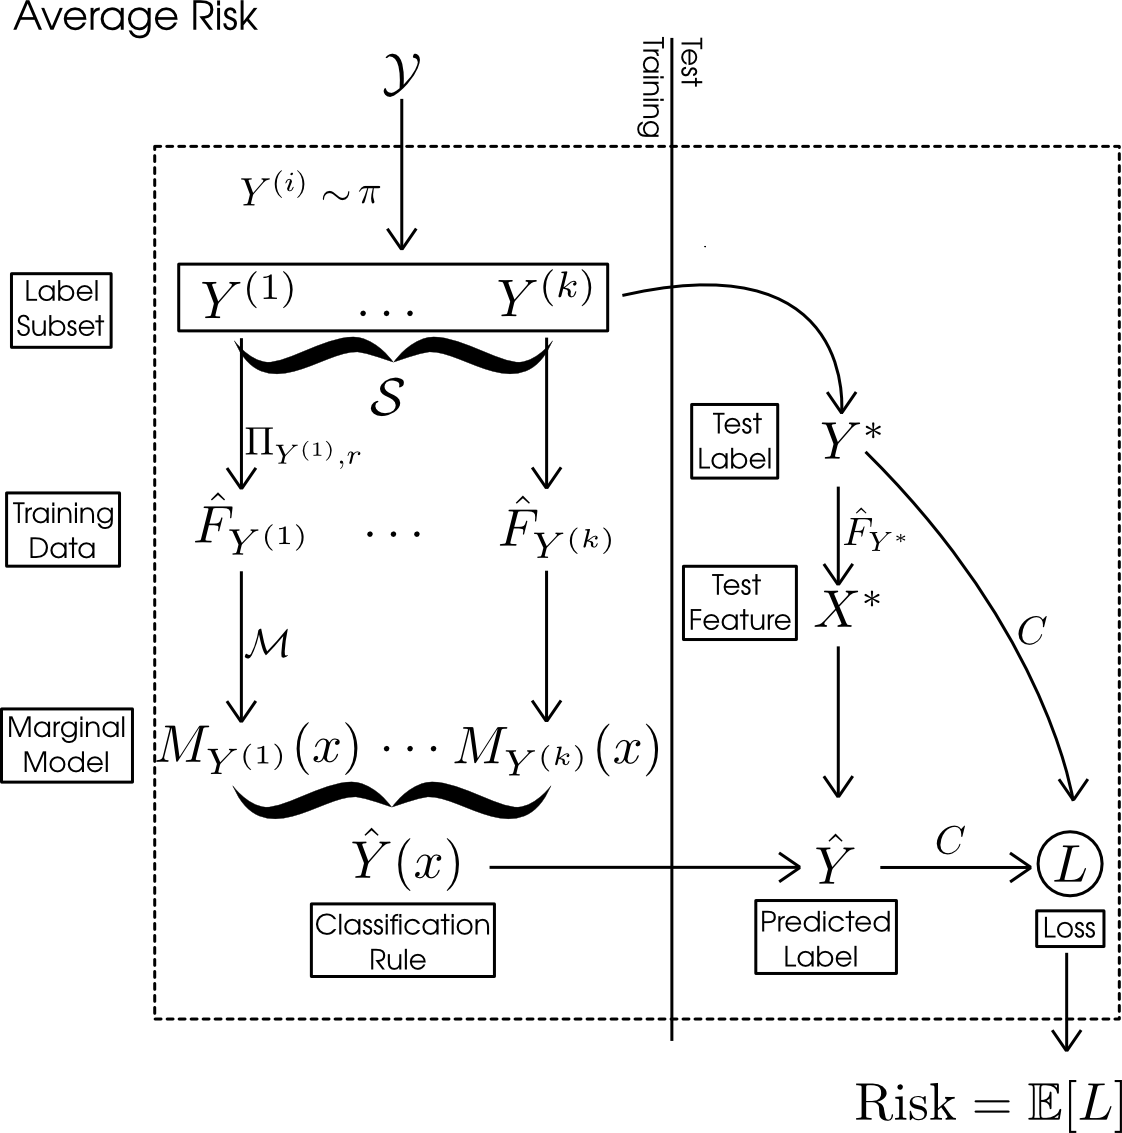
\includegraphics[scale = 0.3]{../extrapolation_figures/average_risk.png}
\caption{Average risk}\label{fig:average_risk2}
\end{figure}

\fi

As we can see from Figure \ref{fig:average_risk}, the average accuracy is
obtained by averaging over four randomizations:
\begin{enumerate}
\item[A1.] Drawing the label subset $\mathcal{S}$.
\item[A2.] Drawing the training dataset.
\item[A3.] Drawing $Y^*$ uniformly at random from $\mathcal{S}$.
\item[A4.] Drawing $X^*$ from $F_{X^*}$.
\end{enumerate}


Our strategy is to analyze the average accuracy by
means of \emph{conditioning on} the true label and its training
sample, $(y^*, \hat{F}_{y^*})$, and the test feature $x^*$
while \emph{averaging} over all the other random variables.  Define
the \emph{conditional accuracy} $\text{CondAcc}_k((y^*, \hat{F}_{y^*}), x^*)$ as
\[
\text{CondAcc}_k((y^*, \hat{F}_{y^*}), x^*) = \Pr[\argmax_{y \in \mathcal{S}} \mathcal{M}(\{\hat{F}_y\})(X^*) = Y^* |Y^*=y^*, X^* = x^*, \hat{F}_{Y^*} = \hat{F}_{y^*}].
\]
Figure \ref{fig:conditional_risk} illustrates the variables which are
fixed under conditioning and the variables which are randomized.
Compare to figure \ref{fig:average_risk}.

Without loss of generality, we can write the label subset $\mathcal{S}
= \{Y^*, Y^{(1)},\hdots, Y^{(k-1)}\}$.  Note that due to independence,
$Y^{(1)},\hdots, Y^{(k-1)}$ are still i.i.d. from $\pi$ even
conditioning on $Y^* = y^*.$ Therefore, the conditional risk can be
obtained via the following alternative order of randomizations:
\begin{enumerate}
\item[C0.] 
Fix $y^*, \hat{F}_y^*,$ and $x^*$.  Note that $M_{y^*}(x^*)
= \mathcal{M}(\hat{F}_{y^*})(x^*)$ is also fixed.
\item[C1.]
Draw the \emph{incorrect labels} $Y^{(1)},\hdots, Y^{(k)}$ i.i.d. from
$\pi$.  (Note that $Y^{(i)} \neq y^*$ with probability 1 due to the
continuity assumptions on $\mathcal{Y}$ and $\pi$.)
\item[C2.]
Draw the training samples for the incorrect labels
$\hat{F}_{Y^{(1)}},\hdots, \hat{F}_{Y^{(k-1)}}$.  This determines
\[
\hat{Y} = \argmax_{y \in \mathcal{S}} M_y(x^*)
\]
and hence, whether or not the classification is correct for $(x^*, y^*)$
\end{enumerate}
Compared to four randomization steps for the average risk, we have
essentially conditioned on steps A3 and A4 and randomized over steps
A1 and A2.

\begin{figure}[h]
\centering
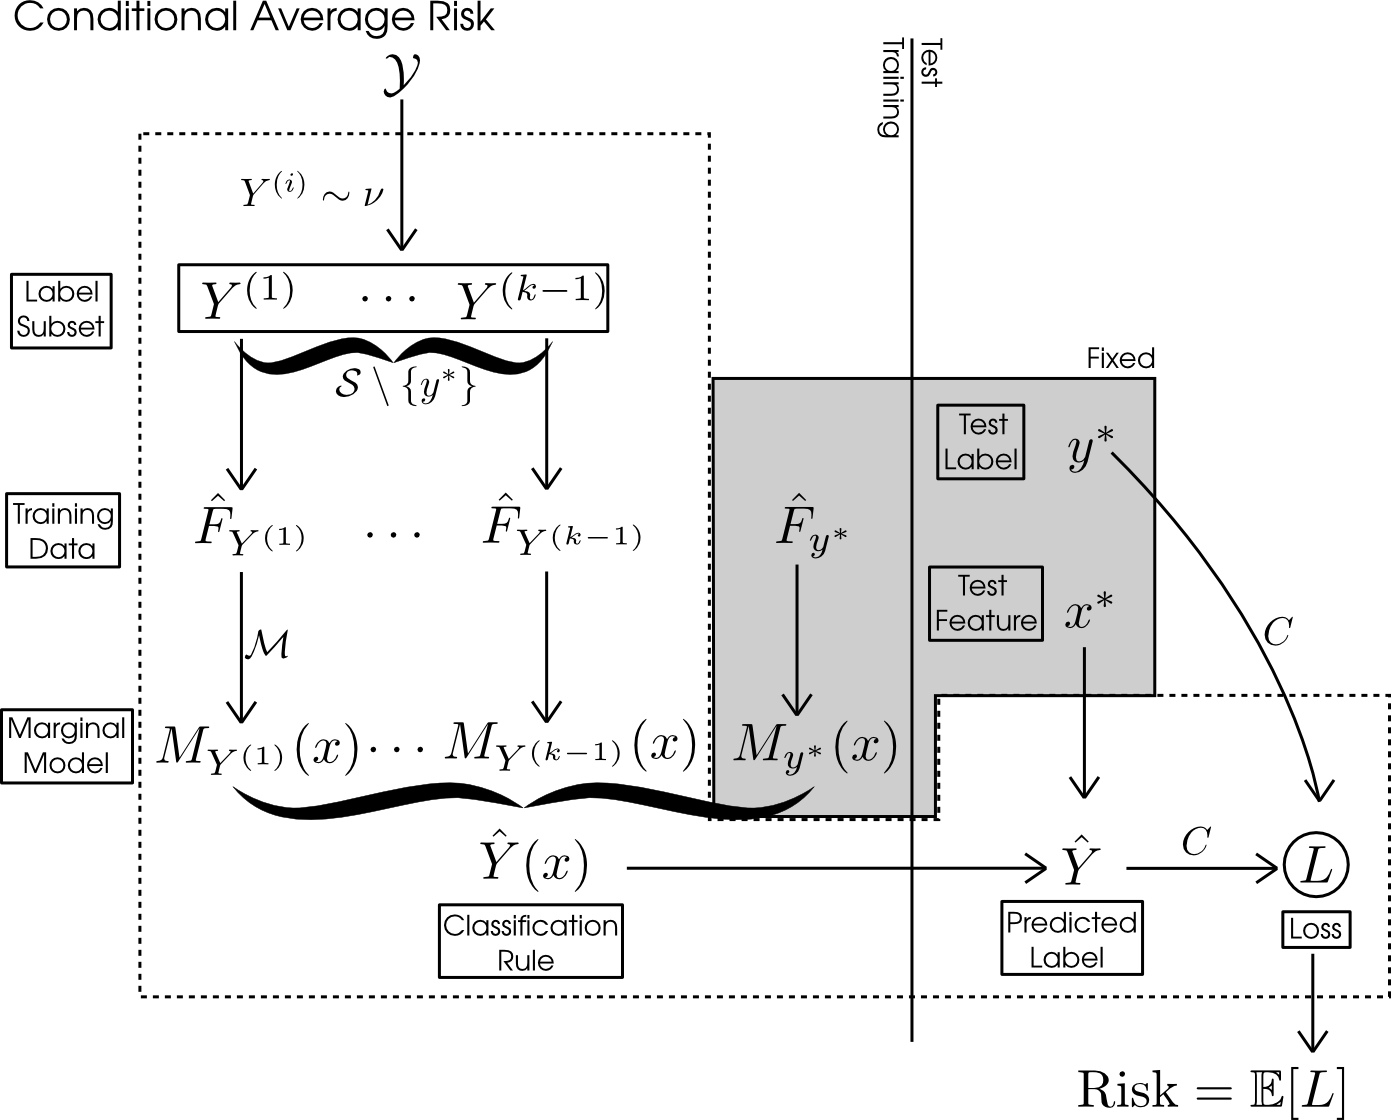
\includegraphics[scale = 0.3]{../extrapolation_figures/conditional_risk.png}
\caption{Conditional accuracy [note: figure needs to be fixed!]}\label{fig:conditional_risk}
\end{figure}

Now, in order to analyze the $k$-class behavior of the conditional
accuracy, we begin by considering the \emph{two-class} situation.

In the two-class situation, we have a true label $y^*$, a training
sample $\hat{F}_{y^*}$, and one incorrect label, $Y$.  Define the
\emph{U-function} $U_{x^*}(y^*, \hat{F}_{y^*})$ as the conditional
accuracy (the probability of correct classification) in the two-class
case.  The classification is correct if the margin $M_{y^*}(x^*)$ is
greater than the margin $M_Y(x^*)$, and incorrect otherwise.  Since we
are fixing $x^*$ and $(y^*, \hat{F}_{y^*})$, the probability of
correct classification is obtained by taking an expectation:
\begin{align}\label{eq:U_function}
U_{x^*}(y^*, \hat{F}_{y^*}) &= \Pr[M_{y^*}(x^*) > \mathcal{M}(\hat{F}_Y)(x^*)]
\\&= \int_{\mathcal{Y}} 
I\{
M_{y^*}(x^*) > \mathcal{M}(\hat{F}_{y})(x)
\}
d\Pi_{y, r}(\hat{F}_y)
d\pi(y).
\end{align}
See also figure \ref{fig:U_function} for an graphical illustration of
the definition.

\begin{figure}[h]
\centering
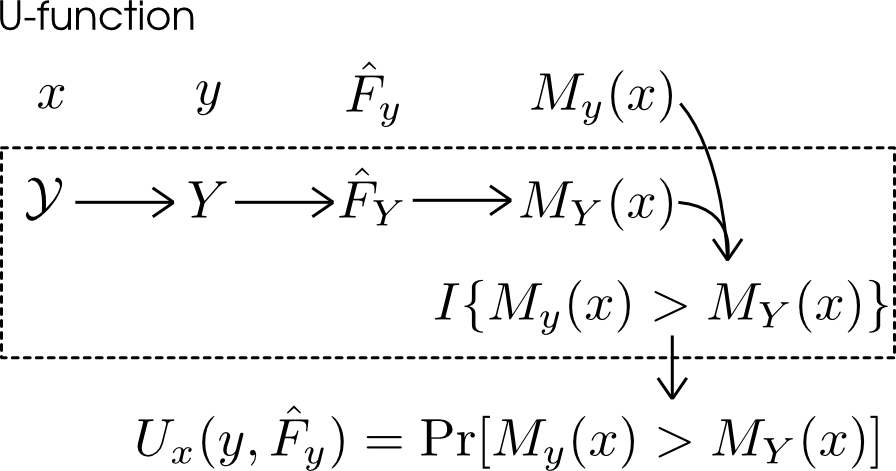
\includegraphics[scale = 0.4]{../extrapolation_figures/U_function.png}
\caption{U-functions}\label{fig:U_function}
\end{figure}

An important property of the U-function, and the basis for its name,
is that the random variable $U_x(Y, \hat{F}_Y)$ for $Y \sim \pi$ and
$\hat{F}_Y \sim \Pi_{Y, r}$ is uniformly distributed for all
$x \in \mathcal{X}$.  This is proved in Lemma \ref{lemma:U_function}
in Appendix C.

Now, we will see how the U-function allows us to understand the
$k$-class case.  Suppose we have true label $y^*$ and incorrect labels
$Y^{(1)},\hdots, Y^{(k-1)}$.  Note that the U-function
$U_{x^*}(y, \hat{F}_y)$ is monotonic in $M_y(x^*)$.  Therefore,
\[
\hat{Y} = \argmax_{y \in \mathcal{S}} M_y(x^*) = \argmax_{y \in \mathcal{S}} U_{x^*}(y, \hat{F}_y).
\]
Therefore, we have a correct classification if and only if the U-function value for the correct label
is greater than the maximum U-function values for the incorrect labels:
\[
\Pr[\hat{Y} = y^*] = \Pr[U_{x^*}(y^*, \hat{F}_{y^*}) > \max_{i=1}^{k-1} U_{x^*}(Y^{(i)}, \hat{F}_{Y^{(i)}})] =  \Pr[u^* > U_{max}].
\]
where $u^* = U_{x^*}(y^*, \hat{F}_{y^*})$ and $U_{max, k-1}
= \max_{i=1}^{k-1} U_{x^*}(Y^{(i)}, \hat{F}_{Y^{(i)}})$.  But now,
observe that we know the distribution of $U_{max, k-1}$!  Since
$U_{x^*}(Y^{(i)}, \hat{F}_{Y^{(i)}})$ are i.i.d. uniform, we know that
\begin{equation}\label{eq:umax_beta}
U_{max, k-1} \sim \text{Beta}(k-1, 1). 
\end{equation}

Therefore, in the general case, the conditional accuracy is
\[
\text{CondAcc}_k((y^*, \hat{F}_{y^*}), x^*) = \Pr[U_{max} > u^*] = 1 - \int_{u^*}^1 (k-1) u^{k-2} du.
\]
Now the average accuracy can be obtained by integrating over the
distribution of $U^* = U_{x^*}(y^*, \hat{F}_{y^*})$, which we state in
the following proof of theorem \ref{theorem:avrisk_identity}.

\noindent\textbf{Proof of Theorem \ref{theorem:avrisk_identity}}.
We have
\begin{align*}
\text{AGA}_{k,r} &= \E[ 1 - \int_{U^*}^1 (k-1) u^{k-2} du] 
\\&= 1 - \E[\int_0^1 I\{u \geq U^*\} (k-1) u^{k-2} du ]
\\&= (k-1) \int_0^1 \Pr[U^* \leq u] u^{k-2} du.
\end{align*}
Or equivalently,
\[
\text{AGA}_{k, r}((y^*, \hat{F}_{y^*}), x^*) = 1 - (k-1) \int \bar{D}(u) u^{k-2} du.
\]
where $\bar{D}(u)$ denotes the cumulative distribution function of $U^*$ on $[0,1]$:
\begin{equation}\label{eq:Kbar}
\bar{D}(u) = \Pr[U_{x^*}(y^*, \hat{F}_{y^*}) \leq u].
\end{equation}
We have expressed the average risk expressed as a weighted integral of
a certain function $\bar{D}(u)$ defined on $u \in [0,1]$.  We have
clearly isolated the part of the average risk which is independent of
$k$--the univariate function $\bar{D}(u)$, and the part which is
dependent on $k$--which is the density of $U_{max}$.

In section \ref{sec:extrapolation_estimation}, we will develop
estimators of $\bar{D}(u)$ in order to estimate the $k$-class average
risk.

Having this theoretical result allows us to understand how the
expected $k$-class risk scales with $k$ in problems where all the
relevant densities are known.  However, applying this result in
practice to estimate $\text{Average Risk}_k$ requires some means of
estimating the unknown function $\bar{D}$--which we discuss in the
following.

\section{Estimation}\label{sec:extrapolation_estimation}

Now we address the problem of estimating $\text{AGA}_{k_2, r_1}$ from
data.  As we have seen from Theorem \ref{theorem:avrisk_identity}, the
$k$-class average accuracy of a marginal classifier $\mathcal{M}$ is a
functional of a object called $\bar{D}(u),$ which depends marginal
model $\mathcal{M}$ of the classifier, the joint distribution of
labels $Y$ and features $X$ when $Y$ is drawn from the sampling
density $\nu$.

Therefore, the strategy we take is to attempt to estimate $\bar{D}$
for then given classification model, and then plug in our estimate of
$\bar{D}$ into the integral \eqref{eq:avrisk_identity} to obtain an
estimate of $\text{AGA}_{k_2, r_{train}}$.

Having decided to estimate $\bar{D}$, there is then the question of
what kind of model we should assume for $\bar{D}$.  In this work, we
assume that some parametric model\footnote{While a
nonparametric approach may be more ideal, we leave this to future work.} is available for $\bar{D}$.

Let us assume the linear model
\begin{equation}\label{eq:linearKu}
\bar{D}(u) = \sum_{\ell = 1}^m \beta_\ell h_\ell(u),
\end{equation}
where $h_\ell(u)$ are known basis functions, and $\beta$ are the model
parameters to be estimated. We can obtain \emph{unbiased} estimation
of $\text{AGA}_{k_2, r_{train}}$ via the unbiased estimates of
$k$-class average risk obtained from \eqref{eq:avtestrisk}.

If we plug in the assumed linear model \eqref{eq:linearKu} into the
identity \eqref{eq:avrisk_identity}, then we get
\begin{align}
1 - \text{AGA}_{k, r_{train}} &= (k-2)\int \bar{D}(u) u^{k-2} du
\\&= (k-2)\int_0^1 \sum_{\ell = 1}^m \beta_\ell h_\ell(u) u^{k-2} du
\\&= \sum_{\ell = 1}^m \beta_\ell H_{\ell,k} \label{eq:avrisk_linear}
\end{align}
where
\begin{equation}
H_{\ell,k} = (k-2) \int_0^1 h_\ell(u) u^{k-2} du.
\end{equation}
The constants $H_{\ell, k}$ are moments of the basis function
$h_\ell$: hence we call this method the \emph{moment method.}  Note
that $H_{\ell, k}$ can be precomputed numerically for any $k \geq 2$.


Now, since the test accuracies $\text{TA}_k$ are unbiased estimates of
$\text{AGA}_{k, r_{train}}$, this implies that the regression
estimate
\[
\hat{\beta} = \argmin_\beta \sum_{k=2}^{k_1} w_k \left( (1 - \text{TA}_k) - \sum_{\ell=1}^m \beta_\ell H_{\ell, k}\right)^2
\]
is unbiased for $\beta$, under any choice of positive weights $w_k$.
The estimate of $\text{AGA}_{k_2,r_1}$ is similarly obtained
from \eqref{eq:avrisk_linear}, via
\begin{equation}\label{eq:avrisk_hat}
\widehat{\text{AGA}_{k_2,r_1}} = \sum_{\ell=1}^m \hat{\beta}_\ell H_{\ell, k_2}.
\end{equation}

\section{Examples}\label{sec:extrapolation_example}

\subsection{Facial recognition example}

From the ``Labeled Faces in the Wild'' dataset (\cite{LFWTech}), we
selected 1672 individuals with at least 2 face photos.  We form a
dataset consisting of photo-label pairs $(\vec{z}_j^{(i)}, y^{(i)})$
for $i = 1,\hdots, 1672$ and $j = 1,2$ by randomly selecting 2 face
photos for each of the 1672 individuals.

We implement a face recognition system based on one nearest-neighbor
and OpenFace (\cite{amos2016openface}) for feature extraction.  For
each photo $\vec{z}$, a 128-dimensional feature vector $\vec{x}$ is
obtained as follows.
\begin{enumerate}
\item The computer vision library DLLib is used to detect landmarks in
  $\vec{z}$, and to apply a nonlinear transformation to align
  $\vec{z}$ to a template.
\item The aligned photograph is downsampled to a $96 \times 96$ input,
  which is fed into a pre-trained deep convolutional neural network to
  obtain the 128-dimensional feature vector $\vec{x}$.
\end{enumerate}
Therefore, we obtain feature-label pairs $(\vec{z}_j^{(i)}, y^{(i)})$
for $i = 1,\hdots, 1672$ and $j = 1,2$.

The recognition system then works as follows.  Suppose we want to
perform facial recognition on a subset of the individuals, $I \subset
\{1,\hdots, 1672\}$.  Then, for all $i \in I$, we load one feature
vector-label pair, into the system, $(\vec{x}_1^{(i)}, y^{(i)})$.  In
order to identify a new photo $\vec{z}^*$, we obtain the feature
vector $\vec{x}^*$, and guess the label $\hat{y}$ based on example
with the minimal distance to $\vec{x}^*$,
\[
\hat{y} = y^{(i^*)}
\]
where
\[
i^* = \text{argmin}_I d(\vec{x}, \vec{x}_1^{(i)}).
\]
The test accuracy is assessed on the unused repeat for all individuals
in $I$.  Note that the assumptions of our estimation method are met in
this example because one-nearest neighbor is a marginal classifier.
One can define the margin functions as
\[
(\mathcal{M}(\vec{x}))(\vec{x}^*) = -||\vec{x} - \vec{x}^*||^2.
\]
However, $k$-nearest neighbor for $k > 1$ is not marginal.

While we can apply our extrapolation method to estimate the average
accuracy for any number of faces $k$, it will not be possible to
validate our estimates if we use the full dataset.  Therefore, we take
the average accuracies computed using the subsampling method
\eqref{eq:avtestrisk} on the full dataset as a \emph{ground truth} to
compare to the average accuracy estimated from a \emph{subsampled}
dataset.  Therefore, we simulate the problem of performance
extrapolation from a database of $K$ faces by subsampling a
dataset of size $K$ from the LFW dataset.

\begin{figure}
\centering
\begin{tabular}{cc}
a & b\\
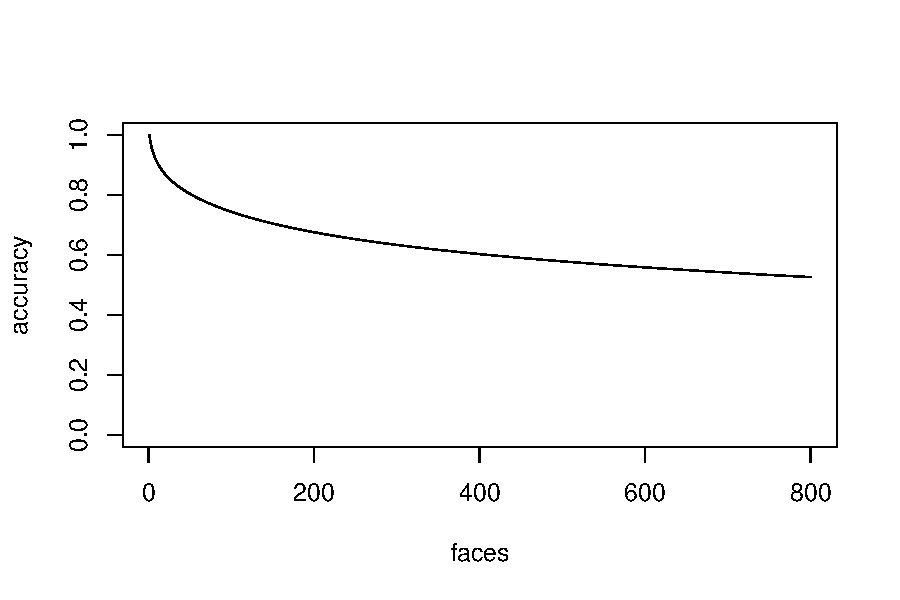
\includegraphics[scale = 0.5]{../../facerec/acc_plot1.pdf} &
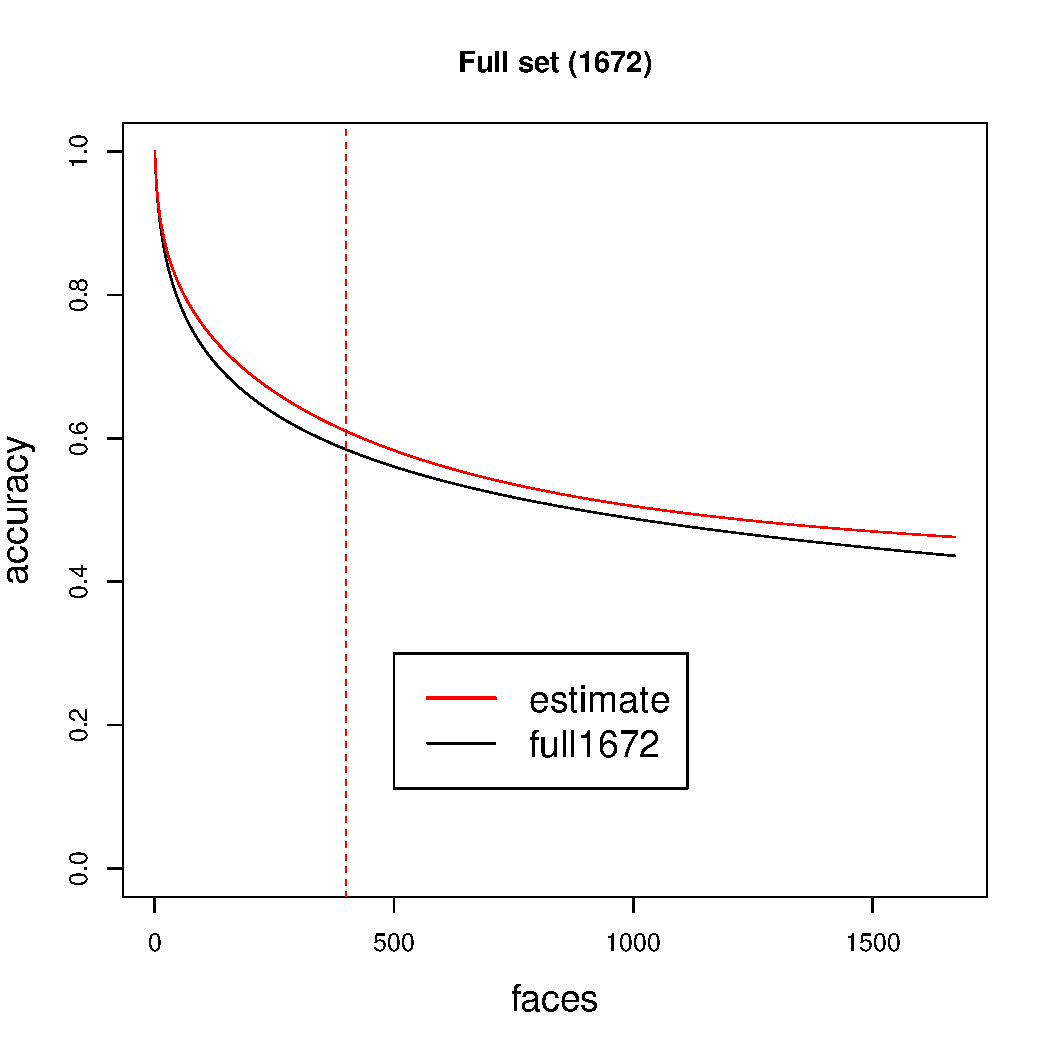
\includegraphics[scale = 0.5]{../../facerec/acc_plot2.pdf}
\end{tabular}
\caption{(a) The estimated average accuracy for $k = 2,\hdots,
  400$ given a dataset of 400 faces subsampled from Labeled Faces in
  the Wild.  (b) Estimated average accuracy for $k > 400$ on the
  same dataset, compared to the ground truth (estimated AGA using all
  1672 classes).}
\label{fig:lfw_extrapolation1}
\end{figure}

To do the performance extrapolation, we use a linear
spline basis,
\[
h_\ell(u) = \left[u - \frac{\ell - 1}{m}\right]_+
\]
for $\ell = 1,\hdots, m$.  Here we take $m = 10000$.  We model the
function $\bar{D}(u)$ as a non-negative linear combination of basis
functions,
\[
\bar{D}(u) = \sum_{\ell = 1}^m \beta_\ell h_\ell(u),
\]
with $\beta_\ell \geq 0$.  The resulting estimated generalization
accuracies, computed using \eqref{eq:avrisk_identity}, are plotted in
Figure \eqref{fig:lfw_extrapolation1} (b).  As we already mentions, to
assess the quality of the estimated average accuracy, we compare them
to the `ground truth' accuracy curve obtained by using all 1672
examples to compute the the average test risk.



To get an idea of the accuracy and variance of the accuracy curve
estimates for varying sample sizes $K$, we repeat this procedure
multiple times for $K \in \{100,200,400, 800\}$.  The results, again
compared to the ground truth computed from the full data set, is
illustrated in figure \ref{fig:lfw_extrapolation2}.

\begin{figure}
\centering
\begin{tabular}{cc}
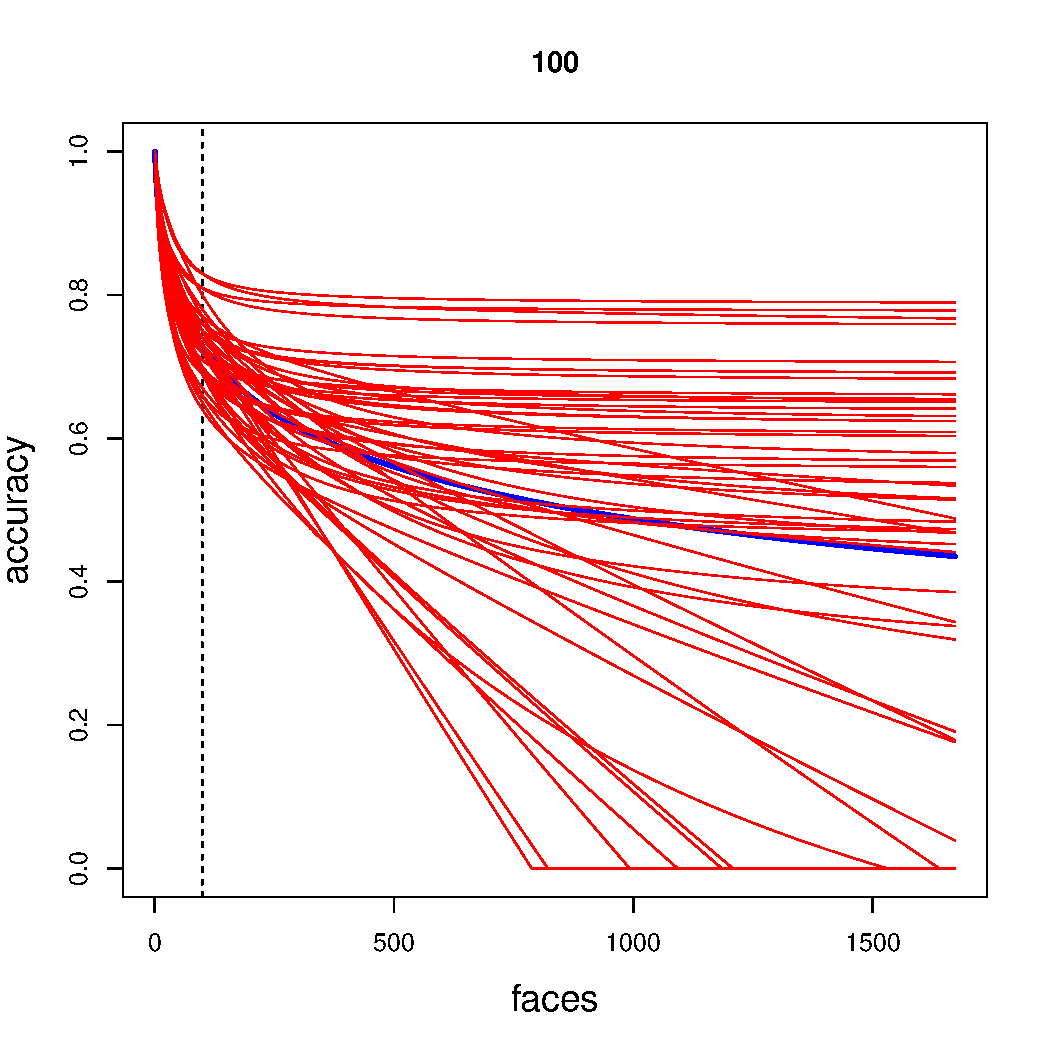
\includegraphics[scale = 0.4]{../../facerec/sub_100.pdf} &
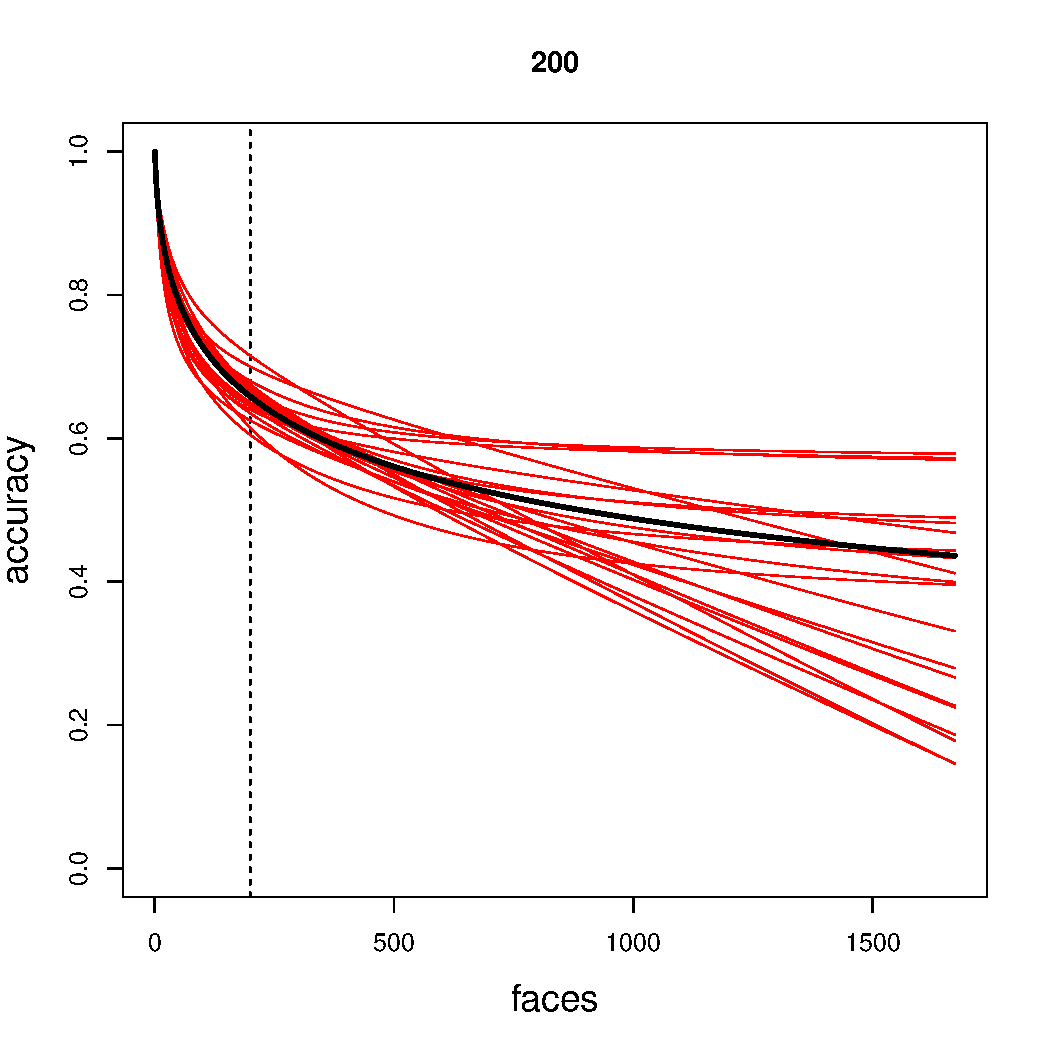
\includegraphics[scale = 0.4]{../../facerec/sub_200.pdf} \\
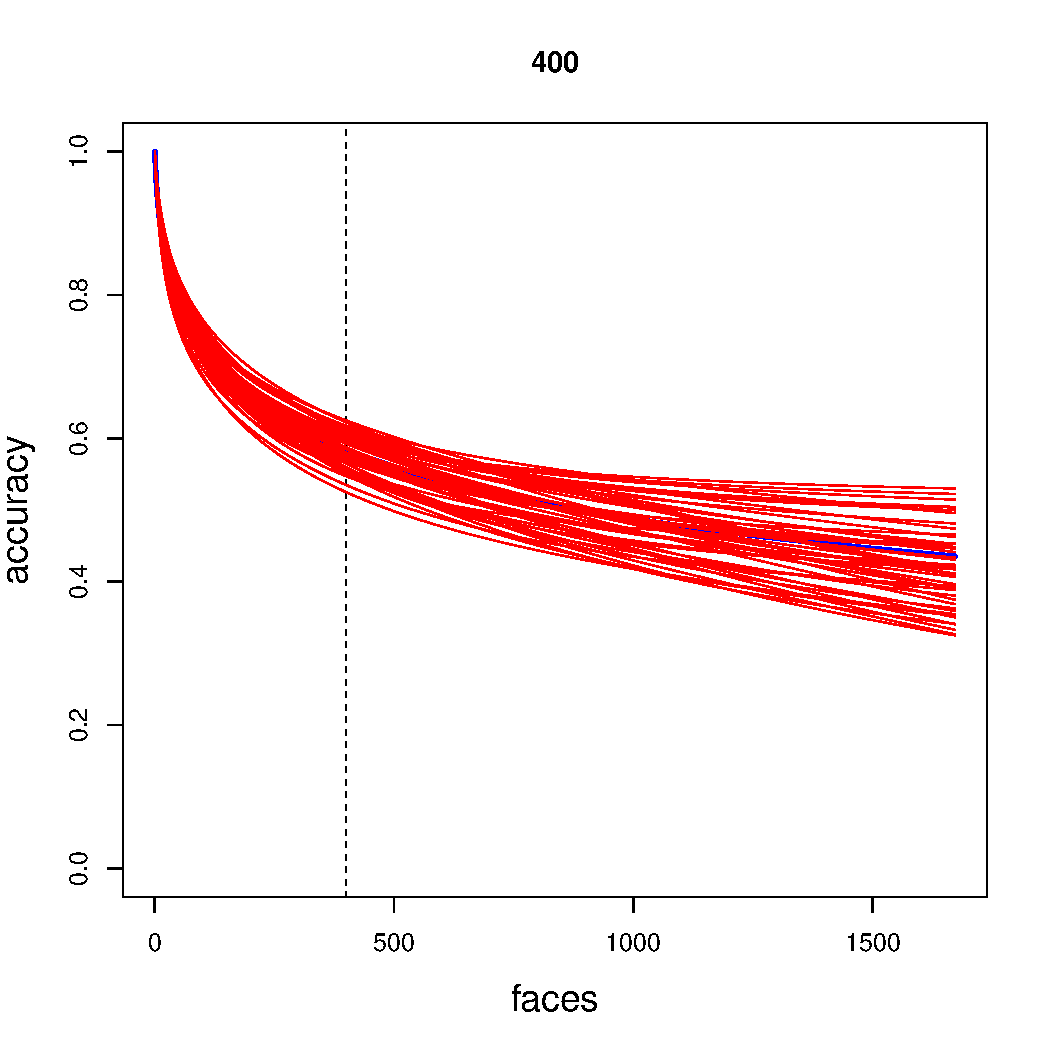
\includegraphics[scale = 0.4]{../../facerec/sub_400.pdf} &
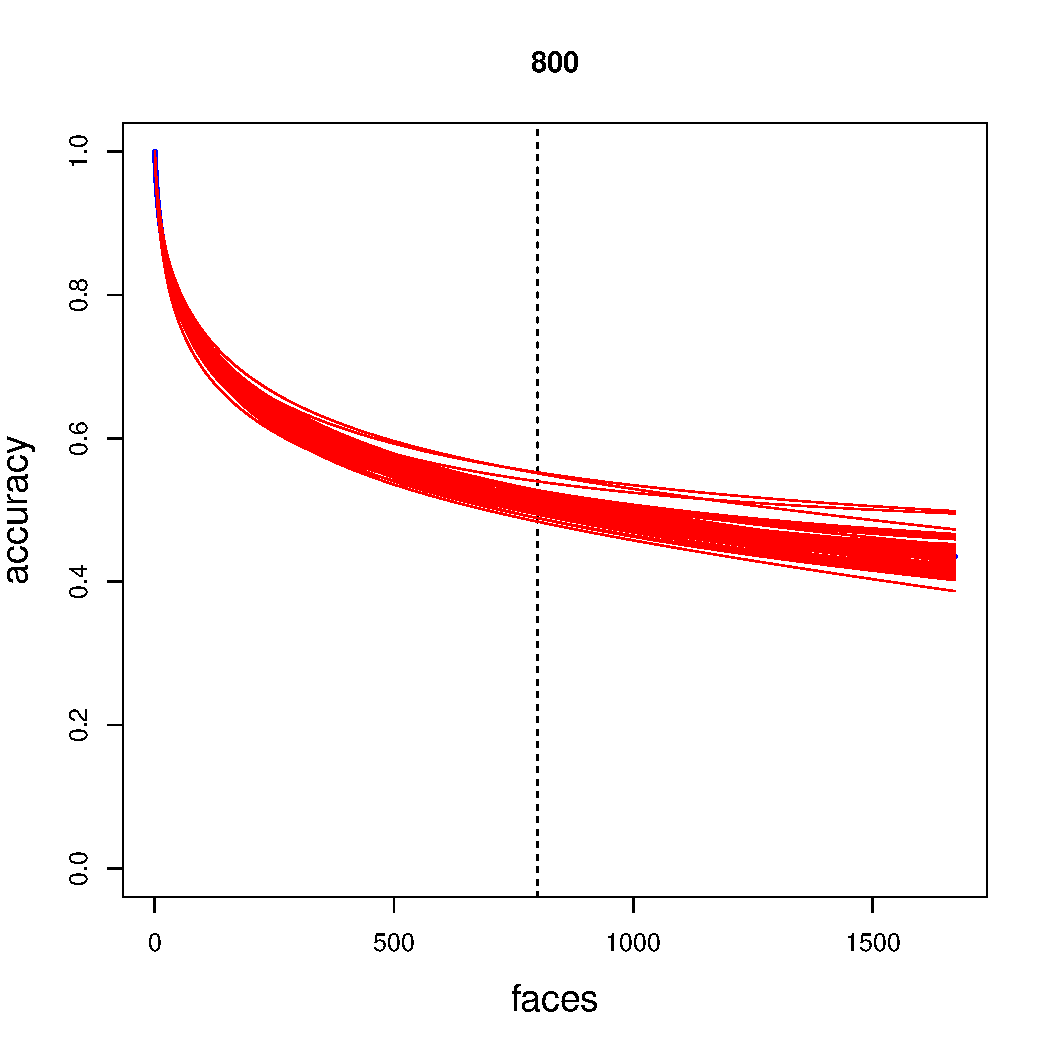
\includegraphics[scale = 0.4]{../../facerec/sub_800.pdf} 
\end{tabular}
\caption{Estimated average accuracy using subsampled datasets of size
  $k$, compared to the ground truth (estimated AGA using all 1672
  classes).}
\label{fig:lfw_extrapolation2}
\end{figure}

\subsection{Telugu OCR example}

While the previous example was a perfect fit to the assumptions of the
framework, we also want to see how well the method works when some of
the assumptions may be violated.  Toward this end we apply performance
extrapolation in an optical character recognition example
(\cite{achanta2015telugu}) for predicting the accuracy on 400 classes
of Telugu characters from a subsample of size $K = 20$.  We consider
the use of five different classifiers: Naive Bayes, logistic
regression, SVM, $\epsilon$-nearest neighbors\footnote{$k$-nearest
  neighbors with $k = \epsilon n$ for fixed $\epsilon > 0$}, and a
deep convolutional neural network\footnote{The network architecture is
  as follows: {\tt
    48x48-4C3-MP2-6C3-8C3-MP2-32C3-50C3-MP2-200C3-SM.}}.  Of the five
classifiers, only Naive Bayes satisfies the marginal classifier
assumption.  Again, we compare the result of our model to the ground
truth obtained by using the full dataset.

\begin{table}
\centering
\begin{tabular}{|c||c|c|c|}\hline
Classifier      & Test $\text{acc}^{(20)}$ & Test $\text{acc}^{(400)}$ & $\hat{AGA}_{400}$ \\ \hline
Naive Bayes     & 0.951                   & 0.601                   & 0.858     \\ \hline
Logistic        & 0.922                   & 0.711                   & 0.812     \\ \hline
SVM             & 0.860                   & 0.545                   & 0.687     \\ \hline
$\epsilon$-NN   & 0.951                   & 0.591                   & 0.410     \\ \hline
Deep neural net & 0.995                   & 0.986                   & 0.907     \\ \hline
\end{tabular}
\caption{Performance extrapolation: predicting the accuracy on 400 classes using data from 20 classes on a Telugu character dataset.
$\epsilon = 0.002$ for $\epsilon$-nearest neighbors.}
\label{tab:telugu}
\end{table}

The results are displayed in Table \ref{tab:telugu}.  To our surprise,
the worst absolute difference between ground truth and estimated
average accuracy was in the case of Naive bayes $(|\delta| = 0.257)$
which satisfies the marginal property.  All other classifiers had
absolute errors less than 0.2.  It is also interesting to note that,
even though Naive Bayes and $\epsilon$-nearest neighbors have the same
test accuracy on the subset, that the predicted accuracy on 400
differs greatly between then (0.858 vs 0.400).  Furthermore, the
difference is in the right direction: Naive Bayes is predicted to work
better on 400 classes than $\epsilon$-nearest neighbors, which appears
to be the case based on the 400-class test accuracy.

While further work is still needed to better understand the
performance of the proposed performance extrapolation method, both for
marginal classifiers (which satisfy the theoretical assumptions) and
non-marginal classifiers (which do not), the results obtained in these
two examples are encouraging in that sense that useful predictions
were obtained both for marginal and non-marginal classifiers.
